\documentclass[twoside]{book}

% Packages required by doxygen
\usepackage{fixltx2e}
\usepackage{calc}
\usepackage{doxygen}
\usepackage[export]{adjustbox} % also loads graphicx
\usepackage{graphicx}
\usepackage[utf8]{inputenc}
\usepackage{makeidx}
\usepackage{multicol}
\usepackage{multirow}
\PassOptionsToPackage{warn}{textcomp}
\usepackage{textcomp}
\usepackage[nointegrals]{wasysym}
\usepackage[table]{xcolor}

% Font selection
\usepackage[T1]{fontenc}
\usepackage[scaled=.90]{helvet}
\usepackage{courier}
\usepackage{amssymb}
\usepackage{sectsty}
\renewcommand{\familydefault}{\sfdefault}
\allsectionsfont{%
  \fontseries{bc}\selectfont%
  \color{darkgray}%
}
\renewcommand{\DoxyLabelFont}{%
  \fontseries{bc}\selectfont%
  \color{darkgray}%
}
\newcommand{\+}{\discretionary{\mbox{\scriptsize$\hookleftarrow$}}{}{}}

% Page & text layout
\usepackage{geometry}
\geometry{%
  a4paper,%
  top=2.5cm,%
  bottom=2.5cm,%
  left=2.5cm,%
  right=2.5cm%
}
\tolerance=750
\hfuzz=15pt
\hbadness=750
\setlength{\emergencystretch}{15pt}
\setlength{\parindent}{0cm}
\setlength{\parskip}{3ex plus 2ex minus 2ex}
\makeatletter
\renewcommand{\paragraph}{%
  \@startsection{paragraph}{4}{0ex}{-1.0ex}{1.0ex}{%
    \normalfont\normalsize\bfseries\SS@parafont%
  }%
}
\renewcommand{\subparagraph}{%
  \@startsection{subparagraph}{5}{0ex}{-1.0ex}{1.0ex}{%
    \normalfont\normalsize\bfseries\SS@subparafont%
  }%
}
\makeatother

% Headers & footers
\usepackage{fancyhdr}
\pagestyle{fancyplain}
\fancyhead[LE]{\fancyplain{}{\bfseries\thepage}}
\fancyhead[CE]{\fancyplain{}{}}
\fancyhead[RE]{\fancyplain{}{\bfseries\leftmark}}
\fancyhead[LO]{\fancyplain{}{\bfseries\rightmark}}
\fancyhead[CO]{\fancyplain{}{}}
\fancyhead[RO]{\fancyplain{}{\bfseries\thepage}}
\fancyfoot[LE]{\fancyplain{}{}}
\fancyfoot[CE]{\fancyplain{}{}}
\fancyfoot[RE]{\fancyplain{}{\bfseries\scriptsize Generated by Doxygen }}
\fancyfoot[LO]{\fancyplain{}{\bfseries\scriptsize Generated by Doxygen }}
\fancyfoot[CO]{\fancyplain{}{}}
\fancyfoot[RO]{\fancyplain{}{}}
\renewcommand{\footrulewidth}{0.4pt}
\renewcommand{\chaptermark}[1]{%
  \markboth{#1}{}%
}
\renewcommand{\sectionmark}[1]{%
  \markright{\thesection\ #1}%
}

% Indices & bibliography
\usepackage{natbib}
\usepackage[titles]{tocloft}
\setcounter{tocdepth}{3}
\setcounter{secnumdepth}{5}
\makeindex

% Hyperlinks (required, but should be loaded last)
\usepackage{ifpdf}
\ifpdf
  \usepackage[pdftex,pagebackref=true]{hyperref}
\else
  \usepackage[ps2pdf,pagebackref=true]{hyperref}
\fi
\hypersetup{%
  colorlinks=true,%
  linkcolor=blue,%
  citecolor=blue,%
  unicode%
}

% Custom commands
\newcommand{\clearemptydoublepage}{%
  \newpage{\pagestyle{empty}\cleardoublepage}%
}

\usepackage{caption}
\captionsetup{labelsep=space,justification=centering,font={bf},singlelinecheck=off,skip=4pt,position=top}

%===== C O N T E N T S =====

\begin{document}

% Titlepage & ToC
\hypersetup{pageanchor=false,
             bookmarksnumbered=true,
             pdfencoding=unicode
            }
\pagenumbering{alph}
\begin{titlepage}
\vspace*{7cm}
\begin{center}%
{\Large Huffman\+Algorithm }\\
\vspace*{1cm}
{\large Generated by Doxygen 1.8.13}\\
\end{center}
\end{titlepage}
\clearemptydoublepage
\pagenumbering{roman}
\tableofcontents
\clearemptydoublepage
\pagenumbering{arabic}
\hypersetup{pageanchor=true}

%--- Begin generated contents ---
\chapter{About Project}
\label{index}\hypertarget{index}{}\hypertarget{index_First}{}\section{Project\textquotesingle{}s aim}\label{index_First}
The aim of this project is to create an application that supports compression and decompression of text files using the Huffman algorithm. When started a menu appears on the screen and the user should input a digit between 1 and 6 in order to choose an action to be performed. The main functionality of the project is to support C\+O\+M\+P\+R\+E\+SS function that takes a file, reads its content and transforms it into a binary string. Moreover when a file is being compressed the compression ratio is printed on the screen whereas the binary sequence including an extra information about the Huffman tree(used when decompressing) are saved in a file. Another functionality is the D\+E\+C\+O\+M\+P\+R\+E\+SS function that takes an already compressed file and creates a new file containing the original content. The next function is called debug. It takes an already compressed file and prints the binary sequence as decimal numbers. When pressing 4 the program terminates. With 5 a text file is taken and compressed. The difference is from option 1 is that the binary sequence is translated into decimal sequence. By pressing 6 the user is able to decompress such files.\hypertarget{index_Github}{}\subsection{Github}\label{index_Github}
\href{https://github.com/bdimitrow/HuffmanAlgorithm}{\tt https\+://github.\+com/bdimitrow/\+Huffman\+Algorithm}\hypertarget{index_Second}{}\section{Compression Ratio}\label{index_Second}
\hypertarget{index_Third}{}\section{Demo}\label{index_Third}
\hypertarget{index_one}{}\subsection{After running}\label{index_one}
\hypertarget{index_two}{}\subsection{Original file content}\label{index_two}
Having a file named \textquotesingle{}test\+Equal.\+txt\textquotesingle{} with the following content\+: \hypertarget{index_three}{}\subsection{Compressed file content}\label{index_three}
The file after being compressed looks like that\+: \hypertarget{index_four}{}\subsection{Decompressed file content}\label{index_four}
The compressed file look like that after the decommpression\+: \hypertarget{index_five}{}\subsection{Debug option output}\label{index_five}
This is the output\+: 
\chapter{Class Index}
\section{Class List}
Here are the classes, structs, unions and interfaces with brief descriptions\+:\begin{DoxyCompactList}
\item\contentsline{section}{\hyperlink{class_huffman_tree}{Huffman\+Tree} \\*A Huffman tree class }{\pageref{class_huffman_tree}}{}
\end{DoxyCompactList}

\chapter{File Index}
\section{File List}
Here is a list of all documented files with brief descriptions\+:\begin{DoxyCompactList}
\item\contentsline{section}{\hyperlink{file_utils_8h}{file\+Utils.\+h} }{\pageref{file_utils_8h}}{}
\item\contentsline{section}{{\bfseries menu.\+h} }{\pageref{menu_8h}}{}
\item\contentsline{section}{\hyperlink{string_utils_8h}{string\+Utils.\+h} }{\pageref{string_utils_8h}}{}
\item\contentsline{section}{\hyperlink{tree_8h}{tree.\+h} }{\pageref{tree_8h}}{}
\end{DoxyCompactList}

\chapter{Class Documentation}
\hypertarget{class_huffman_tree}{}\section{Huffman\+Tree Class Reference}
\label{class_huffman_tree}\index{Huffman\+Tree@{Huffman\+Tree}}


A Huffman tree class.  




{\ttfamily \#include $<$tree.\+h$>$}

\subsection*{Public Member Functions}
\begin{DoxyCompactItemize}
\item 
\hyperlink{class_huffman_tree_a69699f7de5cfcd69e741f72ecb2b043d}{Huffman\+Tree} ()
\item 
\hyperlink{class_huffman_tree_a666b0956e40438a6130f31933271f6c6}{Huffman\+Tree} (const char $\ast$)
\item 
\hyperlink{class_huffman_tree_a610ac7959bfcf17c8a3c02cd9280ef61}{Huffman\+Tree} (std\+::vector$<$ std\+::pair$<$ char, std\+::string $>$$>$ \&)
\item 
\hyperlink{class_huffman_tree_a19a9e458233f8dd7ed99252be797bbd3}{Huffman\+Tree} (const \hyperlink{class_huffman_tree}{Huffman\+Tree} \&)
\item 
\hyperlink{class_huffman_tree}{Huffman\+Tree} \& \hyperlink{class_huffman_tree_a1274cfce54e9bb66af77bff91aa71411}{operator=} (const \hyperlink{class_huffman_tree}{Huffman\+Tree} \&)
\item 
\hyperlink{class_huffman_tree_a1c39382be4e786a99a07183bbee3830d}{$\sim$\+Huffman\+Tree} ()
\item 
bool \hyperlink{class_huffman_tree_acf3a39b33e82f22f88436e6b99809761}{is\+Leaf} (Huffman\+Tree\+Node $\ast$node)
\item 
void \hyperlink{class_huffman_tree_aad4e7b29b81e1b64d1eb48a3bd70747f}{make\+Pairs} (std\+::vector$<$ std\+::pair$<$ char, std\+::string $>$$>$ \&)
\item 
std\+::string \hyperlink{class_huffman_tree_a9089821533c4ef5b1ac5a4f689757603}{decode\+\_\+string} (const std\+::string \&)
\end{DoxyCompactItemize}


\subsection{Detailed Description}
A Huffman tree class. 


\begin{DoxyParams}{Parameters}
{\em root} & is a pointer of type Huffman\+Tree\+Node\\
\hline
\end{DoxyParams}
This class is used to build a Huffman tree from an occurrence table(when compressing) and from string(when decompressing). 

\subsection{Constructor \& Destructor Documentation}
\mbox{\Hypertarget{class_huffman_tree_a69699f7de5cfcd69e741f72ecb2b043d}\label{class_huffman_tree_a69699f7de5cfcd69e741f72ecb2b043d}} 
\index{Huffman\+Tree@{Huffman\+Tree}!Huffman\+Tree@{Huffman\+Tree}}
\index{Huffman\+Tree@{Huffman\+Tree}!Huffman\+Tree@{Huffman\+Tree}}
\subsubsection{\texorpdfstring{Huffman\+Tree()}{HuffmanTree()}\hspace{0.1cm}{\footnotesize\ttfamily [1/4]}}
{\footnotesize\ttfamily Huffman\+Tree\+::\+Huffman\+Tree (\begin{DoxyParamCaption}{ }\end{DoxyParamCaption})}

A default constructor. \mbox{\Hypertarget{class_huffman_tree_a666b0956e40438a6130f31933271f6c6}\label{class_huffman_tree_a666b0956e40438a6130f31933271f6c6}} 
\index{Huffman\+Tree@{Huffman\+Tree}!Huffman\+Tree@{Huffman\+Tree}}
\index{Huffman\+Tree@{Huffman\+Tree}!Huffman\+Tree@{Huffman\+Tree}}
\subsubsection{\texorpdfstring{Huffman\+Tree()}{HuffmanTree()}\hspace{0.1cm}{\footnotesize\ttfamily [2/4]}}
{\footnotesize\ttfamily Huffman\+Tree\+::\+Huffman\+Tree (\begin{DoxyParamCaption}\item[{const char $\ast$}]{str }\end{DoxyParamCaption})\hspace{0.3cm}{\ttfamily [explicit]}}

Constructor for \hyperlink{class_huffman_tree}{Huffman\+Tree} using a char array. Used when compressing a file. The source file is extracted into a char array and the amount of times that each symbol appears is known. Afterwards a Huffman forest is created and stored into a priority queue. The two trees with the smallest amount of occurrences are combined into one tree. When the priority queue has just one element, that element is pointer to the root of the tree. Creating nodes for every symbol with a non-\/zero occurrence and adding it to the queue.\mbox{\Hypertarget{class_huffman_tree_a610ac7959bfcf17c8a3c02cd9280ef61}\label{class_huffman_tree_a610ac7959bfcf17c8a3c02cd9280ef61}} 
\index{Huffman\+Tree@{Huffman\+Tree}!Huffman\+Tree@{Huffman\+Tree}}
\index{Huffman\+Tree@{Huffman\+Tree}!Huffman\+Tree@{Huffman\+Tree}}
\subsubsection{\texorpdfstring{Huffman\+Tree()}{HuffmanTree()}\hspace{0.1cm}{\footnotesize\ttfamily [3/4]}}
{\footnotesize\ttfamily Huffman\+Tree\+::\+Huffman\+Tree (\begin{DoxyParamCaption}\item[{std\+::vector$<$ std\+::pair$<$ char, std\+::string $>$$>$ \&}]{code\+Pairs }\end{DoxyParamCaption})\hspace{0.3cm}{\ttfamily [explicit]}}

Constructor for \hyperlink{class_huffman_tree}{Huffman\+Tree} using a vector of pairs made of char and string. Used when decompressing a file. In a compressed file the Huffman tree is saved as a string that is converted to a vector of pairs of char and string corresponding to that character. The tree is rebuild with this vector. If the string symbol is 0 a left child is created whether there is no one. A similar process happens when the string symbol is 1. However the child is the right one. \mbox{\Hypertarget{class_huffman_tree_a19a9e458233f8dd7ed99252be797bbd3}\label{class_huffman_tree_a19a9e458233f8dd7ed99252be797bbd3}} 
\index{Huffman\+Tree@{Huffman\+Tree}!Huffman\+Tree@{Huffman\+Tree}}
\index{Huffman\+Tree@{Huffman\+Tree}!Huffman\+Tree@{Huffman\+Tree}}
\subsubsection{\texorpdfstring{Huffman\+Tree()}{HuffmanTree()}\hspace{0.1cm}{\footnotesize\ttfamily [4/4]}}
{\footnotesize\ttfamily Huffman\+Tree\+::\+Huffman\+Tree (\begin{DoxyParamCaption}\item[{const \hyperlink{class_huffman_tree}{Huffman\+Tree} \&}]{other }\end{DoxyParamCaption})}

A copy constructor. \mbox{\Hypertarget{class_huffman_tree_a1c39382be4e786a99a07183bbee3830d}\label{class_huffman_tree_a1c39382be4e786a99a07183bbee3830d}} 
\index{Huffman\+Tree@{Huffman\+Tree}!````~Huffman\+Tree@{$\sim$\+Huffman\+Tree}}
\index{````~Huffman\+Tree@{$\sim$\+Huffman\+Tree}!Huffman\+Tree@{Huffman\+Tree}}
\subsubsection{\texorpdfstring{$\sim$\+Huffman\+Tree()}{~HuffmanTree()}}
{\footnotesize\ttfamily Huffman\+Tree\+::$\sim$\+Huffman\+Tree (\begin{DoxyParamCaption}{ }\end{DoxyParamCaption})}

A destructor. 

\subsection{Member Function Documentation}
\mbox{\Hypertarget{class_huffman_tree_a9089821533c4ef5b1ac5a4f689757603}\label{class_huffman_tree_a9089821533c4ef5b1ac5a4f689757603}} 
\index{Huffman\+Tree@{Huffman\+Tree}!decode\+\_\+string@{decode\+\_\+string}}
\index{decode\+\_\+string@{decode\+\_\+string}!Huffman\+Tree@{Huffman\+Tree}}
\subsubsection{\texorpdfstring{decode\+\_\+string()}{decode\_string()}}
{\footnotesize\ttfamily std\+::string Huffman\+Tree\+::decode\+\_\+string (\begin{DoxyParamCaption}\item[{const std\+::string \&}]{binary\+Str }\end{DoxyParamCaption})}


\begin{DoxyParams}{Parameters}
{\em std\+::string} & binary\+Str The function takes the binary string and traverse through the tree. When the string symbol is \textquotesingle{}0\textquotesingle{} the traversal goes to the left child and when it is \textquotesingle{}1\textquotesingle{} the traversal goes to the right child. Reaching a leaf node, the node\textquotesingle{}s symbol is added to the resulting string. When the binary\+Str is exhausted the resulting string is returned. \\
\hline
\end{DoxyParams}
\begin{DoxyReturn}{Returns}
std\+::string result 
\end{DoxyReturn}
\mbox{\Hypertarget{class_huffman_tree_acf3a39b33e82f22f88436e6b99809761}\label{class_huffman_tree_acf3a39b33e82f22f88436e6b99809761}} 
\index{Huffman\+Tree@{Huffman\+Tree}!is\+Leaf@{is\+Leaf}}
\index{is\+Leaf@{is\+Leaf}!Huffman\+Tree@{Huffman\+Tree}}
\subsubsection{\texorpdfstring{is\+Leaf()}{isLeaf()}}
{\footnotesize\ttfamily bool Huffman\+Tree\+::is\+Leaf (\begin{DoxyParamCaption}\item[{Huffman\+Tree\+Node $\ast$}]{node }\end{DoxyParamCaption})\hspace{0.3cm}{\ttfamily [inline]}}

Checks whether a node is a leaf(it has no children). 
\begin{DoxyParams}{Parameters}
{\em Huffman\+Tree\+Node} & $\ast$node \\
\hline
\end{DoxyParams}
\begin{DoxyReturn}{Returns}
bool 
\end{DoxyReturn}
\mbox{\Hypertarget{class_huffman_tree_aad4e7b29b81e1b64d1eb48a3bd70747f}\label{class_huffman_tree_aad4e7b29b81e1b64d1eb48a3bd70747f}} 
\index{Huffman\+Tree@{Huffman\+Tree}!make\+Pairs@{make\+Pairs}}
\index{make\+Pairs@{make\+Pairs}!Huffman\+Tree@{Huffman\+Tree}}
\subsubsection{\texorpdfstring{make\+Pairs()}{makePairs()}}
{\footnotesize\ttfamily void Huffman\+Tree\+::make\+Pairs (\begin{DoxyParamCaption}\item[{std\+::vector$<$ std\+::pair$<$ char, std\+::string $>$$>$ \&}]{vec }\end{DoxyParamCaption})}

Uses the private function make\+Pairs to create vector of pairs for the public. \mbox{\Hypertarget{class_huffman_tree_a1274cfce54e9bb66af77bff91aa71411}\label{class_huffman_tree_a1274cfce54e9bb66af77bff91aa71411}} 
\index{Huffman\+Tree@{Huffman\+Tree}!operator=@{operator=}}
\index{operator=@{operator=}!Huffman\+Tree@{Huffman\+Tree}}
\subsubsection{\texorpdfstring{operator=()}{operator=()}}
{\footnotesize\ttfamily \hyperlink{class_huffman_tree}{Huffman\+Tree} \& Huffman\+Tree\+::operator= (\begin{DoxyParamCaption}\item[{const \hyperlink{class_huffman_tree}{Huffman\+Tree} \&}]{other }\end{DoxyParamCaption})}

An operator =. That copies the \textquotesingle{}other\textquotesingle{} tree to \textquotesingle{}this\textquotesingle{} tree. 

The documentation for this class was generated from the following files\+:\begin{DoxyCompactItemize}
\item 
\hyperlink{tree_8h}{tree.\+h}\item 
tree.\+cpp\end{DoxyCompactItemize}

\chapter{File Documentation}
\hypertarget{file_utils_8h}{}\section{file\+Utils.\+h File Reference}
\label{file_utils_8h}\index{file\+Utils.\+h@{file\+Utils.\+h}}
{\ttfamily \#include \char`\"{}tree.\+h\char`\"{}}\newline
{\ttfamily \#include \char`\"{}string\+Utils.\+h\char`\"{}}\newline
{\ttfamily \#include $<$iostream$>$}\newline
{\ttfamily \#include $<$fstream$>$}\newline
{\ttfamily \#include $<$sstream$>$}\newline
{\ttfamily \#include $<$cmath$>$}\newline
{\ttfamily \#include $<$iomanip$>$}\newline
Include dependency graph for file\+Utils.\+h\+:\nopagebreak
\begin{figure}[H]
\begin{center}
\leavevmode
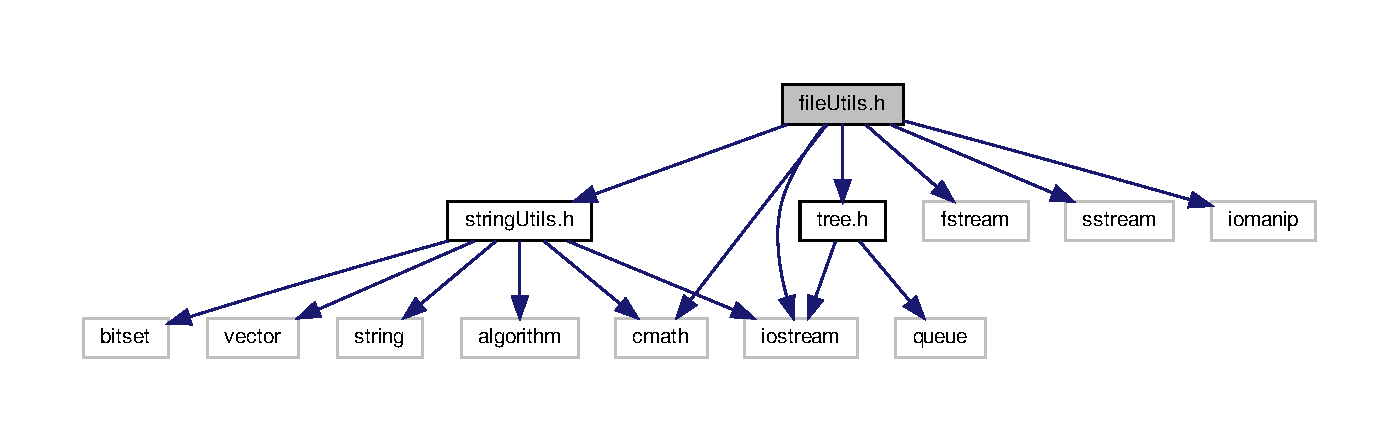
\includegraphics[width=350pt]{file_utils_8h__incl}
\end{center}
\end{figure}
This graph shows which files directly or indirectly include this file\+:\nopagebreak
\begin{figure}[H]
\begin{center}
\leavevmode
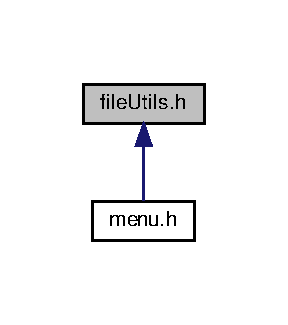
\includegraphics[width=138pt]{file_utils_8h__dep__incl}
\end{center}
\end{figure}
\subsection*{Functions}
\begin{DoxyCompactItemize}
\item 
std\+::string \hyperlink{file_utils_8h_a238a8662b6612f89b672ef5bb5208702}{read\+Whole\+File} (const std\+::string \&file\+Open\+Name)
\item 
void \hyperlink{file_utils_8h_a41239797cbfecd902f7c9bf42a826481}{read\+File\+For\+Decompress} (const std\+::string \&file\+Name, std\+::string \&bintree, std\+::string \&code)
\item 
void \hyperlink{file_utils_8h_aec61ed4ac6aca80ba5a1fcbe45ad4bfa}{read\+File\+For\+Decimal\+Decompress} (const std\+::string \&file\+Name, std\+::string \&bintree, std\+::string \&code)
\item 
void \hyperlink{file_utils_8h_af308c6c14f3c243c5ef73c03d88154e9}{save\+String\+To\+File} (const std\+::string \&file\+Name, const std\+::string \&for\+Storage)
\item 
void \hyperlink{file_utils_8h_a5bdd7b506a387c0a22cc8a84b003bc57}{compare\+Sizes} (const std\+::string \&original\+Content, const std\+::string \&encoded)
\end{DoxyCompactItemize}


\subsection{Function Documentation}
\mbox{\Hypertarget{file_utils_8h_a5bdd7b506a387c0a22cc8a84b003bc57}\label{file_utils_8h_a5bdd7b506a387c0a22cc8a84b003bc57}} 
\index{file\+Utils.\+h@{file\+Utils.\+h}!compare\+Sizes@{compare\+Sizes}}
\index{compare\+Sizes@{compare\+Sizes}!file\+Utils.\+h@{file\+Utils.\+h}}
\subsubsection{\texorpdfstring{compare\+Sizes()}{compareSizes()}}
{\footnotesize\ttfamily void compare\+Sizes (\begin{DoxyParamCaption}\item[{const std\+::string \&}]{original\+Content,  }\item[{const std\+::string \&}]{encoded }\end{DoxyParamCaption})}

This function takes two strings as arguments. The first one is the whole content of a file before compressing and the second one is the content compressed. The function calculates the bytes of both and compares them. The result is printed on the console. 
\begin{DoxyParams}{Parameters}
{\em const} & std\+::string \&original\+Content \\
\hline
{\em const} & std\+::string \&encoded \\
\hline
\end{DoxyParams}
Here is the caller graph for this function\+:\nopagebreak
\begin{figure}[H]
\begin{center}
\leavevmode
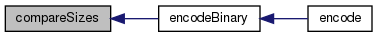
\includegraphics[width=350pt]{file_utils_8h_a5bdd7b506a387c0a22cc8a84b003bc57_icgraph}
\end{center}
\end{figure}
\mbox{\Hypertarget{file_utils_8h_aec61ed4ac6aca80ba5a1fcbe45ad4bfa}\label{file_utils_8h_aec61ed4ac6aca80ba5a1fcbe45ad4bfa}} 
\index{file\+Utils.\+h@{file\+Utils.\+h}!read\+File\+For\+Decimal\+Decompress@{read\+File\+For\+Decimal\+Decompress}}
\index{read\+File\+For\+Decimal\+Decompress@{read\+File\+For\+Decimal\+Decompress}!file\+Utils.\+h@{file\+Utils.\+h}}
\subsubsection{\texorpdfstring{read\+File\+For\+Decimal\+Decompress()}{readFileForDecimalDecompress()}}
{\footnotesize\ttfamily void read\+File\+For\+Decimal\+Decompress (\begin{DoxyParamCaption}\item[{const std\+::string \&}]{file\+Name,  }\item[{std\+::string \&}]{bintree,  }\item[{std\+::string \&}]{code }\end{DoxyParamCaption})}

This function is used for decimal decompression. The file with name \textquotesingle{}file\+Name\textquotesingle{} is opened if there such a file. The file content is extracted into a string \textquotesingle{}whole\+Content\textquotesingle{}. This stirng is splitted into three parts. \textquotesingle{}last\+Size\textquotesingle{} which denotes the number of bits the last number should be. Then comes the information needed for rebuilding the tree. And the \textquotesingle{}code\+Numbers\textquotesingle{} part which is changed from decimal to binary sequence(\textquotesingle{}code\textquotesingle{}). The \textquotesingle{}bintree\textquotesingle{} and \textquotesingle{}code\textquotesingle{} are returned as reference arguments. 
\begin{DoxyParams}{Parameters}
{\em const} & std\+::string \&file\+Name \\
\hline
{\em std\+::string} & \&bintree \\
\hline
{\em std\+::string} & \&code \\
\hline
\end{DoxyParams}
Here is the call graph for this function\+:\nopagebreak
\begin{figure}[H]
\begin{center}
\leavevmode
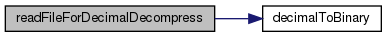
\includegraphics[width=350pt]{file_utils_8h_aec61ed4ac6aca80ba5a1fcbe45ad4bfa_cgraph}
\end{center}
\end{figure}
Here is the caller graph for this function\+:\nopagebreak
\begin{figure}[H]
\begin{center}
\leavevmode
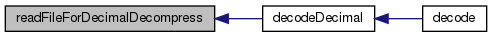
\includegraphics[width=350pt]{file_utils_8h_aec61ed4ac6aca80ba5a1fcbe45ad4bfa_icgraph}
\end{center}
\end{figure}
\mbox{\Hypertarget{file_utils_8h_a41239797cbfecd902f7c9bf42a826481}\label{file_utils_8h_a41239797cbfecd902f7c9bf42a826481}} 
\index{file\+Utils.\+h@{file\+Utils.\+h}!read\+File\+For\+Decompress@{read\+File\+For\+Decompress}}
\index{read\+File\+For\+Decompress@{read\+File\+For\+Decompress}!file\+Utils.\+h@{file\+Utils.\+h}}
\subsubsection{\texorpdfstring{read\+File\+For\+Decompress()}{readFileForDecompress()}}
{\footnotesize\ttfamily void read\+File\+For\+Decompress (\begin{DoxyParamCaption}\item[{const std\+::string \&}]{file\+Name,  }\item[{std\+::string \&}]{bintree,  }\item[{std\+::string \&}]{code }\end{DoxyParamCaption})}

This function is used for binary decompression. The file with name \textquotesingle{}filename\textquotesingle{} is opened if there is such a file. The file content is extracted into a string \textquotesingle{}whole\+Content\textquotesingle{}. Then this string is divided into two parts. The first one \textquotesingle{}bintree\textquotesingle{} contains the needed information to rebuild the tree. The second one is called \textquotesingle{}code\textquotesingle{} and holds the binary sequence. The two parts are returned as reference arguments. 
\begin{DoxyParams}{Parameters}
{\em const} & std\+::string \&file\+Name \\
\hline
{\em std\+::string} & \&bintree \\
\hline
{\em std\+::string} & \&code \\
\hline
\end{DoxyParams}
Here is the caller graph for this function\+:\nopagebreak
\begin{figure}[H]
\begin{center}
\leavevmode
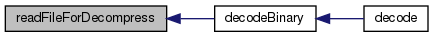
\includegraphics[width=350pt]{file_utils_8h_a41239797cbfecd902f7c9bf42a826481_icgraph}
\end{center}
\end{figure}
\mbox{\Hypertarget{file_utils_8h_a238a8662b6612f89b672ef5bb5208702}\label{file_utils_8h_a238a8662b6612f89b672ef5bb5208702}} 
\index{file\+Utils.\+h@{file\+Utils.\+h}!read\+Whole\+File@{read\+Whole\+File}}
\index{read\+Whole\+File@{read\+Whole\+File}!file\+Utils.\+h@{file\+Utils.\+h}}
\subsubsection{\texorpdfstring{read\+Whole\+File()}{readWholeFile()}}
{\footnotesize\ttfamily std\+::string read\+Whole\+File (\begin{DoxyParamCaption}\item[{const std\+::string \&}]{file\+Open\+Name }\end{DoxyParamCaption})}

The function takes a string(name of the file to be opened) as an argument and returns the whole file content in a string. 
\begin{DoxyParams}{Parameters}
{\em const} & std\+::string \&file\+Open\+Name \\
\hline
\end{DoxyParams}
\begin{DoxyReturn}{Returns}
std\+::string file\+Content 
\end{DoxyReturn}
Here is the caller graph for this function\+:\nopagebreak
\begin{figure}[H]
\begin{center}
\leavevmode
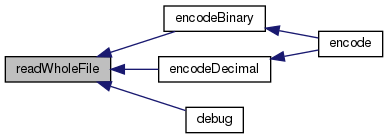
\includegraphics[width=350pt]{file_utils_8h_a238a8662b6612f89b672ef5bb5208702_icgraph}
\end{center}
\end{figure}
\mbox{\Hypertarget{file_utils_8h_af308c6c14f3c243c5ef73c03d88154e9}\label{file_utils_8h_af308c6c14f3c243c5ef73c03d88154e9}} 
\index{file\+Utils.\+h@{file\+Utils.\+h}!save\+String\+To\+File@{save\+String\+To\+File}}
\index{save\+String\+To\+File@{save\+String\+To\+File}!file\+Utils.\+h@{file\+Utils.\+h}}
\subsubsection{\texorpdfstring{save\+String\+To\+File()}{saveStringToFile()}}
{\footnotesize\ttfamily void save\+String\+To\+File (\begin{DoxyParamCaption}\item[{const std\+::string \&}]{file\+Name,  }\item[{const std\+::string \&}]{for\+Storage }\end{DoxyParamCaption})}

The function opens the file with \textquotesingle{}file\+Name\textquotesingle{} name and save the \textquotesingle{}for\+Storage\textquotesingle{} string it in if the opening was successful. 
\begin{DoxyParams}{Parameters}
{\em const} & std\+::string \&file\+Name \\
\hline
{\em const} & std\+::string \&for\+Storage \\
\hline
\end{DoxyParams}
Here is the caller graph for this function\+:\nopagebreak
\begin{figure}[H]
\begin{center}
\leavevmode
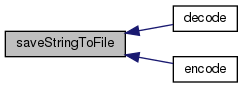
\includegraphics[width=254pt]{file_utils_8h_af308c6c14f3c243c5ef73c03d88154e9_icgraph}
\end{center}
\end{figure}

\hypertarget{string_utils_8h}{}\section{string\+Utils.\+h File Reference}
\label{string_utils_8h}\index{string\+Utils.\+h@{string\+Utils.\+h}}
{\ttfamily \#include $<$iostream$>$}\newline
{\ttfamily \#include $<$vector$>$}\newline
{\ttfamily \#include $<$cmath$>$}\newline
{\ttfamily \#include $<$string$>$}\newline
{\ttfamily \#include $<$algorithm$>$}\newline
{\ttfamily \#include $<$bitset$>$}\newline
Include dependency graph for string\+Utils.\+h\+:\nopagebreak
\begin{figure}[H]
\begin{center}
\leavevmode
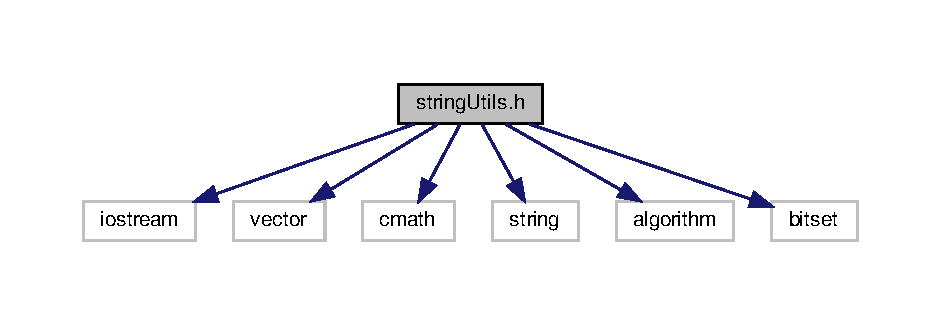
\includegraphics[width=350pt]{string_utils_8h__incl}
\end{center}
\end{figure}
This graph shows which files directly or indirectly include this file\+:\nopagebreak
\begin{figure}[H]
\begin{center}
\leavevmode
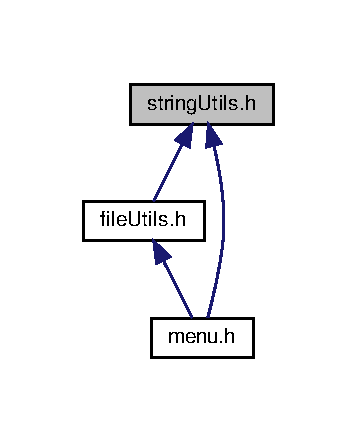
\includegraphics[width=172pt]{string_utils_8h__dep__incl}
\end{center}
\end{figure}
\subsection*{Functions}
\begin{DoxyCompactItemize}
\item 
std\+::string \hyperlink{string_utils_8h_a95ab5c9436cf673dab142534b3d9d2b8}{encode\+String} (std\+::string real\+Content, std\+::vector$<$ std\+::pair$<$ char, std\+::string $>$$>$ \&code\+Pairs)
\item 
std\+::string \hyperlink{string_utils_8h_aba807da1e1e845d2803bbd298e4c7835}{vector\+Code\+Pairs\+To\+String} (std\+::vector$<$ std\+::pair$<$ char, std\+::string $>$$>$ \&code\+Pairs)
\item 
\mbox{\Hypertarget{string_utils_8h_a90dc5a9e01b32661b88d228809f3faa2}\label{string_utils_8h_a90dc5a9e01b32661b88d228809f3faa2}} 
std\+::vector$<$ std\+::pair$<$ char, std\+::string $>$ $>$ {\bfseries string\+To\+Vector\+Code\+Pairs} (std\+::string pair\+Str)
\item 
std\+::string \hyperlink{string_utils_8h_a94956b3add0021210707c7118df76fc3}{binary\+To\+Decimal} (std\+::string binary)
\item 
std\+::string \hyperlink{string_utils_8h_a07ac52f96c548c3dd23dc8674429caae}{decimal\+To\+Binary} (const std\+::string \&binary)
\item 
std\+::string \hyperlink{string_utils_8h_a331f0ff71d04ffc7bc071784035c81d7}{content\+As\+Numbers} (const std\+::string \&binary\+Content)
\end{DoxyCompactItemize}


\subsection{Function Documentation}
\mbox{\Hypertarget{string_utils_8h_a94956b3add0021210707c7118df76fc3}\label{string_utils_8h_a94956b3add0021210707c7118df76fc3}} 
\index{string\+Utils.\+h@{string\+Utils.\+h}!binary\+To\+Decimal@{binary\+To\+Decimal}}
\index{binary\+To\+Decimal@{binary\+To\+Decimal}!string\+Utils.\+h@{string\+Utils.\+h}}
\subsubsection{\texorpdfstring{binary\+To\+Decimal()}{binaryToDecimal()}}
{\footnotesize\ttfamily std\+::string binary\+To\+Decimal (\begin{DoxyParamCaption}\item[{std\+::string}]{binary }\end{DoxyParamCaption})}

Transforming a string(storing binary number) into a string(storing a decimal number). \mbox{\Hypertarget{string_utils_8h_a331f0ff71d04ffc7bc071784035c81d7}\label{string_utils_8h_a331f0ff71d04ffc7bc071784035c81d7}} 
\index{string\+Utils.\+h@{string\+Utils.\+h}!content\+As\+Numbers@{content\+As\+Numbers}}
\index{content\+As\+Numbers@{content\+As\+Numbers}!string\+Utils.\+h@{string\+Utils.\+h}}
\subsubsection{\texorpdfstring{content\+As\+Numbers()}{contentAsNumbers()}}
{\footnotesize\ttfamily std\+::string content\+As\+Numbers (\begin{DoxyParamCaption}\item[{const std\+::string \&}]{binary\+Content }\end{DoxyParamCaption})}

Takes a string consisting just of 0s and 1s. Splits the string into substrings of length == 8 and transforms this 8 bits binary number into decimal ones. Returns them as a string. 
\begin{DoxyParams}{Parameters}
{\em std\+::string} & binary\+Content \\
\hline
\end{DoxyParams}
\begin{DoxyReturn}{Returns}
std\+::string numeric\+Content 
\end{DoxyReturn}
\mbox{\Hypertarget{string_utils_8h_a07ac52f96c548c3dd23dc8674429caae}\label{string_utils_8h_a07ac52f96c548c3dd23dc8674429caae}} 
\index{string\+Utils.\+h@{string\+Utils.\+h}!decimal\+To\+Binary@{decimal\+To\+Binary}}
\index{decimal\+To\+Binary@{decimal\+To\+Binary}!string\+Utils.\+h@{string\+Utils.\+h}}
\subsubsection{\texorpdfstring{decimal\+To\+Binary()}{decimalToBinary()}}
{\footnotesize\ttfamily std\+::string decimal\+To\+Binary (\begin{DoxyParamCaption}\item[{const std\+::string \&}]{binary }\end{DoxyParamCaption})}

Transforming a string(storing a decimal number) into a string(storing a binary number -\/ 8 bits long). \mbox{\Hypertarget{string_utils_8h_a95ab5c9436cf673dab142534b3d9d2b8}\label{string_utils_8h_a95ab5c9436cf673dab142534b3d9d2b8}} 
\index{string\+Utils.\+h@{string\+Utils.\+h}!encode\+String@{encode\+String}}
\index{encode\+String@{encode\+String}!string\+Utils.\+h@{string\+Utils.\+h}}
\subsubsection{\texorpdfstring{encode\+String()}{encodeString()}}
{\footnotesize\ttfamily std\+::string encode\+String (\begin{DoxyParamCaption}\item[{std\+::string}]{real\+Content,  }\item[{std\+::vector$<$ std\+::pair$<$ char, std\+::string $>$$>$ \&}]{code\+Pairs }\end{DoxyParamCaption})}

This function accepts string and vector of pairs(char, string) as arguments. The string in the pair is the binary code for the char. The result is a binary sequence of the real content. 
\begin{DoxyParams}{Parameters}
{\em std\+::string} & real\+Content \\
\hline
{\em std\+::vector$<$std\+::pair$<$char,std\+::string$>$$>$} & \&code\+Pairs \\
\hline
\end{DoxyParams}
\begin{DoxyReturn}{Returns}
std\+::string binary\+Sequence 
\end{DoxyReturn}
\mbox{\Hypertarget{string_utils_8h_aba807da1e1e845d2803bbd298e4c7835}\label{string_utils_8h_aba807da1e1e845d2803bbd298e4c7835}} 
\index{string\+Utils.\+h@{string\+Utils.\+h}!vector\+Code\+Pairs\+To\+String@{vector\+Code\+Pairs\+To\+String}}
\index{vector\+Code\+Pairs\+To\+String@{vector\+Code\+Pairs\+To\+String}!string\+Utils.\+h@{string\+Utils.\+h}}
\subsubsection{\texorpdfstring{vector\+Code\+Pairs\+To\+String()}{vectorCodePairsToString()}}
{\footnotesize\ttfamily std\+::string vector\+Code\+Pairs\+To\+String (\begin{DoxyParamCaption}\item[{std\+::vector$<$ std\+::pair$<$ char, std\+::string $>$$>$ \&}]{code\+Pairs }\end{DoxyParamCaption})}

Transforming vector of pairs into a string. 
\begin{DoxyParams}{Parameters}
{\em std\+::vector$<$std\+::pair$<$char,std\+::string$>$$>$} & code\+Pairs \\
\hline
\end{DoxyParams}
\begin{DoxyReturn}{Returns}
std\+::string pair\+Str 
\end{DoxyReturn}

\hypertarget{tree_8h}{}\section{tree.\+h File Reference}
\label{tree_8h}\index{tree.\+h@{tree.\+h}}
{\ttfamily \#include $<$iostream$>$}\newline
{\ttfamily \#include $<$queue$>$}\newline
Include dependency graph for tree.\+h\+:\nopagebreak
\begin{figure}[H]
\begin{center}
\leavevmode
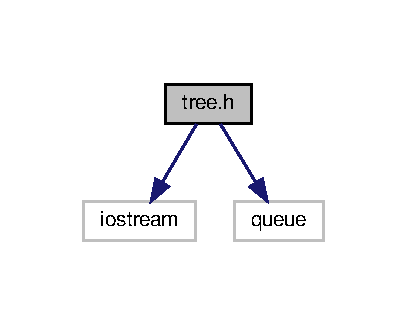
\includegraphics[width=196pt]{tree_8h__incl}
\end{center}
\end{figure}
This graph shows which files directly or indirectly include this file\+:\nopagebreak
\begin{figure}[H]
\begin{center}
\leavevmode
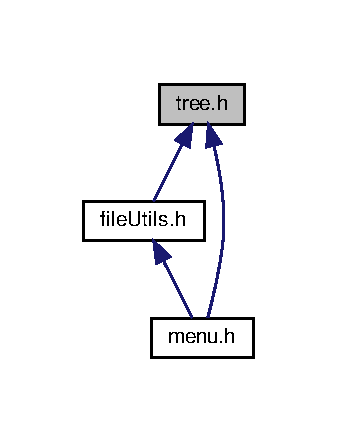
\includegraphics[width=162pt]{tree_8h__dep__incl}
\end{center}
\end{figure}
\subsection*{Classes}
\begin{DoxyCompactItemize}
\item 
class \hyperlink{class_huffman_tree}{Huffman\+Tree}
\begin{DoxyCompactList}\small\item\em A Huffman tree class. \end{DoxyCompactList}\end{DoxyCompactItemize}

\chapter{Example Documentation}
\hypertarget{01111-example}{}\section{01111}
-\/$>$ \char`\"{}15\char`\"{} 
\begin{DoxyParams}{Parameters}
{\em std\+::string} & binary \\
\hline
\end{DoxyParams}
\begin{DoxyReturn}{Returns}
std\+::string decimal
\end{DoxyReturn}

\begin{DoxyCodeInclude}
\end{DoxyCodeInclude}
 
\hypertarget{15-example}{}\section{15}
-\/$>$ \char`\"{}00001111\char`\"{} 
\begin{DoxyParams}{Parameters}
{\em std\+::string} & decimal \\
\hline
\end{DoxyParams}
\begin{DoxyReturn}{Returns}
std\+::string binary
\end{DoxyReturn}

\begin{DoxyCodeInclude}
\end{DoxyCodeInclude}
 
%--- End generated contents ---

% Index
\backmatter
\newpage
\phantomsection
\clearemptydoublepage
\addcontentsline{toc}{chapter}{Index}
\printindex

\end{document}
